The wPCC has wind-assisted ship propulsion (WASP) and can alter between a fully sailing mode, and a fully motoring mode, and in between. 
However, this paper only considers the motoring mode. Because of the WASP, the wPCC design differs slightly from conventional motoring cargo ship designs. The wPCC has two very large rudders, two to three times larger than needed for a conventional ship. The ship also has fins at the bilge to generate extra lift while sailing, as shown on the scale model in \autoref{fig:wPCC}. 
%This figure also show two fans, that can be used to simulate wind forces, these were however not used in the manoeuvring tests of this paper. 
\autoref{tab:main_particulars} shows the main particulars of the scale model. 
\begin{figure}[h]
    \centering
    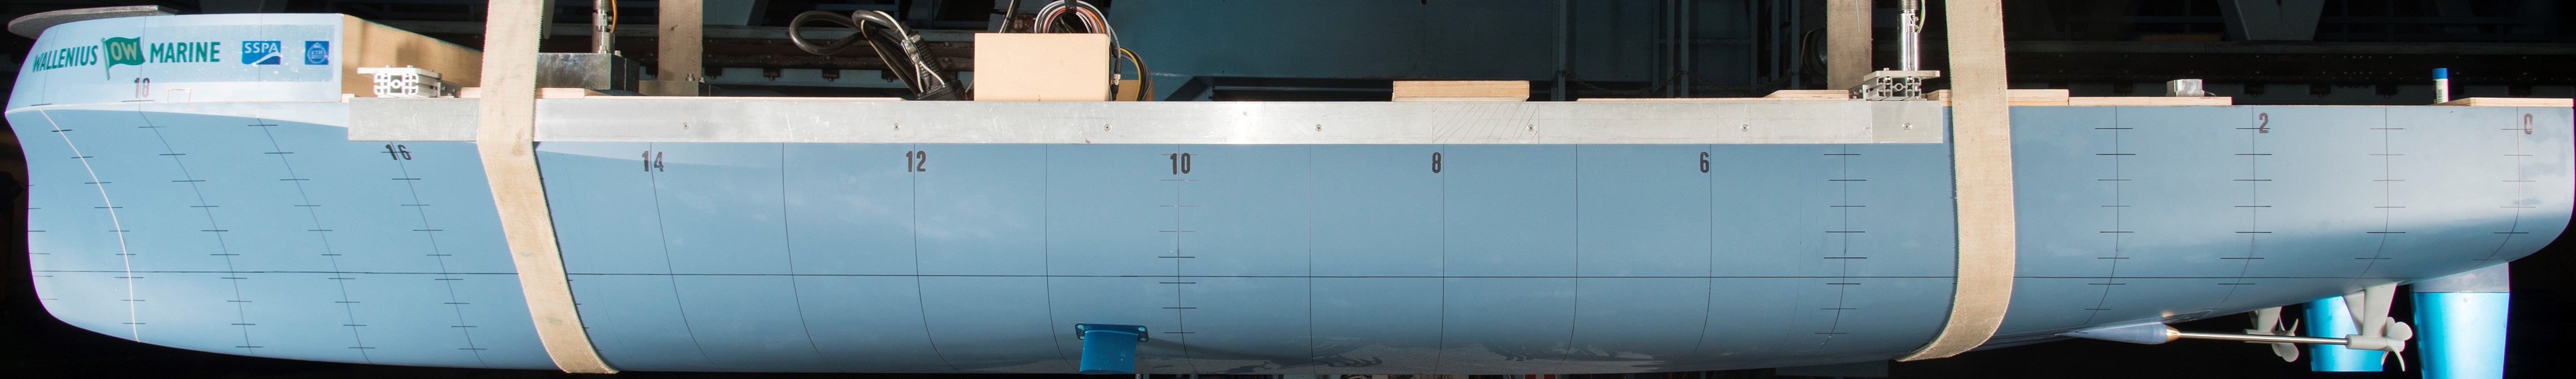
\includegraphics[width=\columnwidth]{figures/5m2.jpg}
    \caption{Scale model of the wPCC used in the model tests. Copyright RISE.}
    \label{fig:wPCC}
\end{figure}

Required input parameters for the semi-empirical rudder model are summarized in \autoref{tab:other_parameters}.
The rudder areas where obtained according to \autoref{fig:rudder_coverage}.   
Some manual tuning of the rudder drag was necessary, especially in the neutral rudder case, where the drag was increased almost eight times, as shown by $C_{D0tune}$. The rudder hull interaction coefficient $a_H$ was set to 0.12, indicating that 12\% of the rudder force is generated on the ship hull.
Rudder angles greater than 15 degrees ($\delta_{lim}$) were assumed to be affected by the gap between rudder and rudder horn with an estimated strength $s$ based on experience from similar rudder arrangements.
The local inflow to the rudders $\gamma_{0port},\gamma_{0stbd}$ was set to $\pm 2.5$ degrees to produce zero lift in the straight-ahead condition.
The added mass coefficients are shown in \autoref{tab:added_masses}.
\begin{table}[h]
    \centering
    \caption{Main particulars (SI units) of the wPCC scale model.}
    \label{tab:main_particulars}
    \pgfplotstabletypeset[col sep=comma, column type=r,
        columns/Parameter/.style={column type=l,string type},
        columns/Unit/.style={column type=l,string type,column name=~},
        columns/Description/.style={column type=l,string type},
        columns/Value/.style={column type=r, column name=~},
        every head row/.style={before row=\hline,after row=\hline},
        every last row/.style={after row=\hline}
    ]{tables/result_models.main_particulars.csv}
\end{table}